\section{Crashkurs}
\label{section:crashkurs}
Wir beginnen mit einem Überblick der grundlegende Bausteine.
In den nachfolgenden Kapiteln besprechen wir einige der Bausteine nochmal im Detail.


\subsection{Kommentare}
\label{section:crashkurs:kommentare}
Kommentare in \Python beginnen mit \lpy{#} und enden am Ende der Zeile.
Sie verhalten sich also ganz genau wie Kommentare in \CC, die mit \lcpp{//} beginnen%
\footnote{Die Kommentare \lcpp{//} wurden in \CNeunundneunzig (siehe \cite{C99}) eingeführt.}.
Gut platzierte Kommentare dürfen in keinem Programm fehlen.
Ein schlecht kommentiertes Programm ist ein Anzeichen dafür, dass es von einem schlechten Programmierer geschrieben wurde.


\subsection{Print}
\label{section:crashkurs:print}
So gut wie alle Objekte können durch die \Python Funktion \lpy{print} auf der Standardausgabe ausgegeben werden.
Das liegt daran, dass die meisten Objekte Klassen sind und die Funktion \lpy{__str__} implementieren (auch wenn wir das jetzt noch nicht verstehen; siehe Abschnitt \ref{section:klassen:spezielle_funktionen}).
Die Funktion \lpy{print} ist für \PythonZwei und \PythonDrei verschieden.
\begin{lstlisting}
print 'Hallo', 'Welt'   # Python2
print ('Hallo', 'Welt') # Python3
\end{lstlisting}
In diesem Skript nutzen wir die von \PythonDrei bereitgestellte Version von \lpy{print}.
Will man in \PythonZwei die \lpy{print}-Funktion aus \PythonDrei verwenden, kann man folgende Zeile am Anfang seines Skript einfügen.
\begin{lstlisting}
from __future__ import print_function # Nutze Python3-print in Python2
\end{lstlisting}


\subsection{Typ und Identität}
\label{section:crashkurs:typ_und_id}
Um die Identiät eines Objekts \lpy{x} zu bestimmen, nutzen wir die Funktion \lpy{id(x)}.
Sie gibt einen String zurück, den wir mit \lpy{print} ausdrucken können.
Ganz ähnlich bekommen wir den Typ eines Objekts mit \lpy{type(x)}.


\subsection{Zahlen}
\label{section:crashkurs:zahlen}
In \Python gibt es die Zahlentypen \lpy{int}, \lpy{long}, \lpy{float} und \lpy{complex}.
Sie verhalten sich (fast) genauso wie die aus \CC bekannten Typen \lcpp{int}, \lcpp{long}, \lcpp{float} und \lcpp{complex}%
\footnote{Der Typ \lpy{complex} wurde in \CNeunundneunzig (siehe \cite{C99}) eingeführt.}.
Man erstellt ein Objekt vom Typ \lpy{int}, durch Angabe einer ganzen Zahl oder durch Aufrufen der Funktion \lpy{int}.
Ähnlich erstellt man ein Objekt vom Typ \lpy{float}, durch Angabe einer Kommazahl oder durch Aufrufen der Funktion \lpy{float}.
\begin{lstlisting}
print( 2 )        # 2    typ: int
print( int(2.1) ) # 2    typ: int
print( 2.0 )      # 2.0  typ: float
print( float(2) ) # 2.0  typ: float
\end{lstlisting}
Man kann zwei verschiedene oder gleiche Zahlentypen mit mathematischen Operatoren verbinden.
Das Ergebnis hat den ``genaueren'' Typ.
Des Weiteren beschreibt \lpy{//} die ganzzahlige Division ohne Rest.
\begin{lstlisting}
print( 2 + 3.3 )  # 5.3  typ: int +  float -> float
print( 5 // 2 )   # 2    typ: int // int   -> int
print( 5.3 // 2 ) # 2.0  typ: int // float -> float
\end{lstlisting}
Die Division von Ganzzahlen unterscheidet sich in \PythonZwei und \PythonDrei.
\begin{lstlisting}
4 /  2 # Python2: 2 vom Typ int;   Python3: 2.0 vom Typ float;
4 // 2 # Python2: 2 vom Typ int;   Python3: 2   vom Typ int;
\end{lstlisting}


\subsection{Strings}
\label{section:crashkurs:strings}
Strings die eine Zeile lang sind, werden entweder mit \lpy{'} oder mit \lstinline[style=PyInline]|"| begonnen und beendet.
Soll ein String mehre Zeilen lang sein, kann man ihn mit \lstinline[style=PyInline]|"""| beginnen und beenden.
Genau wie in \CC gibt es gewisse Zeichen, die nicht direkt geschrieben werden können und mit \lstinline[language=C++,style=CPP]|\| beginnen müssen (zum Beispiel werden neue Zeilen durch \lstinline[language=C++,style=CPP]|\n| ausgedrückt).
Folgender Code erstellt den String ``Hallo[Neue Zeile]Welt''.
\begin{lstlisting}
print( 'Hallo\nWelt' ) # Hallo[neue Zeile]Welt
\end{lstlisting}
Es gibt eine große Auswahl an Funktionen, um aus einem gegebenen String einen neuen zu erstellen.
Beispielsweise verknüpft man zwei Strings mit \lpy{+} und die Funktion \lpy{lower} ersetzt alle Großbuchstaben durch Kleinbuchstaben.
\begin{lstlisting}
print( 'Hallo' + ' ' + 'Welt' ) # Hallo Welt
print( 'Hallo Welt'.lower() )   # hallo welt
\end{lstlisting}


\subsection{Bedingungen}
\label{section:crashkurs:bedingungen}
In \Python gibt es genau zwei Objekte \lpy{True} und \lpy{False} von Typ \lpy{bool}.
(Fast) alle Typen können mit der Funktion \lpy{bool} in einen der beiden Objekte umgewandelt werden.
Den Kontrollfluss des Programms steuert man im einfachsten Fall wir folgt.
\begin{lstlisting}
if bedingung:
  ausdruck
  ...
\end{lstlisting}
Das heißt, wir brauchen zunächst eine Expression \lpy{bedingung}, die als \lpy{True} oder \lpy{False} interpretiert werden kann.
Wertet sie als \lpy{True} aus, so wird ein Block von Ausdrücken ausgeführt.
Anders als in \CC werden in \Python Blöcke nicht durch Klammern, sondern durch konsistente Einrückung definiert.
\begin{lstlisting}
x = 101//3+46//5
if x == 42:
  print('Die Antwort')
\end{lstlisting}
Da gut eingerückter Code (also Code, in dem jeder Block konsistent eingerückt ist) deutlich lesbarer sind als nicht eingerückter
Code, ist er in jedem Fall -- unabhängig von der Sprache -- ein Zeichen für eine gute Programmiererin. 

Da es jedoch trotzdem immer noch genug Leute gibt, die hässlichen Code produzieren, wird man in \Python dazu gezwungen, auf 
konsistente Einrückung zu achten: zu einem Block gehören genau die nachfolgenden Zeilen, die genauso weit eingerückt sind wie die 
erste Zeile des Blocks. Bei nicht konsistenter Einrückung gibt es Syntaxfehler. Dies macht es sehr schwer, hässlichen Code in
\Python zu schreiben.

Aus eigener Erfahrung können wir sagen, dass man sich als erfahrene \CC Programmiererin recht schnell an diese Konvention gewöhnen kann, 
wenn man auch schon vorher auf sauber geschriebene Programme geachtet hat.

Optional besteht eine Bedingung aus keinem oder mehreren \lpy{elif bedingung:}\footnote{sprich ``else if''} und keinem oder einem \lpy{else:}
Die Konstrukte \lpy{else:} und \lpy{elif bedingung:} in \Python verhalten sich wie die Konstrukte \lcpp{else} und \lcpp{else if} in \CC.
\begin{lstlisting}
x = 101//3+46//5               # x = ?
if x == 42:                    # Falls x den Wert 42 hat:
  print('Die Antwort')         # Drucke 'Die Antwort'
elif x == 84:                  # Sonst, falls x den Wert 84 hat:
  print('Zweimal die Antwort') # Drucke 'Zweimal die Antwort'
elif x == 106:                 # Sonst, falls x den Wert 106 hat:
  print('Dreimal die Antwort') # Drucke 'Dreimal die Antwort'
else:                          # In allen anderen Faellen:
  print('Versuchs nochmal')    # Drucke 'Versuchs nochmal'
\end{lstlisting}


\subsection{Listen}
\label{section:crashkurs:listen}
In \Python gibt es verschiedene ``Containertypen'' und hier besprechen wir den Typ \lpy{list}.
Eine Liste \lpy{thor} ist eine linear geordnete Menge von Variablen, auf die man mit \lpy{thor[0], thor[1], ..., thor[i]} zugreift.
Um auf Elemente von hinten zuzugreifen, sind negative Werte für \lpy{i} erlaubt.
\begin{lstlisting}
thor = [2, 'Hallo', 33.3, 'Welt', [] ] # Erzeugt eine Liste
print( thor[1], thor[-1] )             # Gibt folgendes aus: Hallo []
\end{lstlisting}
Die Länge einer Liste ist \lpy{len(thor)}.
Listen sind mutable, das heißt wir können sie verändern.
Mit \lpy{thor.append(x)} erweitert man die Liste \lpy{thor} um die Variable \lpy{x} und mit \lpy{thor.remove(x)} entfernt man die erste Variable mit dem Wert \lpy{x}.
Ob ein Objekt mit Wert \lpy{x} in \lpy{thor} enthalten ist, testet man mit \lpy{x in thor}.
Mit \lpy{thor+asgard} verknüpft man die beiden Listen \lpy{thor} und \lpy{asgard}.


\subsection{Schleifen}
\label{section:crashkurs:schleifen}
In \Python gibt es zwei Arten von Schleifen.
Die \lpy{while}-Schleife führt einen Codeblock aus, solange die vor der Ausführung des Blocks geprüfte Bedingung als \lpy{True} auswertet.
\begin{lstlisting}
while bedingung:
  ausdruck
  ...
\end{lstlisting}
Da uns dieses Konzept aus \CC sehr vertraut ist, brauchen wir hier kein Beispiel.

Die \lpy{for}-Schleife führt einen Codeblock für jedes Element einer gegebenen Sequenz (siehe Abschnitt \ref{section:std_data_types:sequenzen}) aus.
Eine Sequenz kann zum Beispiel eine Liste oder ein String sein.
\begin{lstlisting}
for i in s: # der Ausdruck s muss als Sequenz interpretiert werden koennen
  ausdruck
  ...
\end{lstlisting}
Dabei referenziert die Laufvariable \lpy{i} jedes Element der Sequenz \lpy{s} nacheinander einmal. Durch Verwendung von \lpy{i} innerhalb 
des folgenden Codeblocks kann 
dann auf den Wert des jeweiligen Objekts zugegriffen werden. Nach Ausführung des Codeblocks der \lpy{for}-Schleife referenziert 
\lpy{i} dann das nächste Element von \lpy{s}, bis das Ende der Sequenz erreicht ist. 

Dies wird durch das folgende Beispiel veranschaulicht:
\begin{lstlisting}
s = 'Hallo Welt' # Die Sequenz 'Hallo Welt'
for i in s:      # Nimm alle i = H,a,l,l,o, ,W,e,l,t
  print(i)       # Drucke i aus
\end{lstlisting}
Hier ist unsere Sequenz \lpy{s} ein String mit dem Wert \lpy{Hallo Welt}. In der \lpy{for}-Schleife nimmt die Laufvariable nacheinander
die Werte der einzelnen Zeichen von \lpy{s}, also \lpy{H,a,l,} \lpy{l,o, ,W,e,l} und \lpy{t}. Im zur Schleife gehörenden Block werden 
diese Zeichen dann einzeln ausgegeben.

Wenn der Codeblock für eine aufsteigende Folge von Zahlen \lpy{from, from+1, ..., to-1} ausgeführt werden soll, nimmt man die Sequenz \lpy{range(from, to)}.
Wichtig ist, dass wir das halboffene Interval betrachten, also nur bis \lpy{to-1} und nicht bis \lpy{to} gehen.
Damit verhält sich der \Python-Code \lpy{for i in range(from, to):} ganz genau wie der \CC-Code \lstinline[language=C++,style=CPPinline]|for(i = from; i < to; ++i) { ... }|.
Hier ein Beispiel
\begin{lstlisting}
sum = 0              # Setze sum auf 0
for i in range(1,5): # Nimm alle i = 1, 2, 3, 4
  sum += 3*i         # Addiere 3*i zu sum
print( sum )         # Drucke sum aus
\end{lstlisting}

Will man eine absteigende Folge ganzer Zahlen, oder allgemeiner eine Folge ganzer Zahlen mit Schrittweite \lpy{step > 0} oder \lpy{step < 0} haben,
nimmt man die Sequenz \lpy{range(from,to,step)}.
Also können wir obiges Beispiel wie folgt umformulieren.
\begin{lstlisting}
sum = 0                  # Setze sum auf 0
for i in range(3,15, 3): # Nimm alle i = 3, 6, 9, 12
  sum += i               # Addiere i zu sum
print( sum )             # Drucke sum aus
\end{lstlisting}


\subsection{Funktionen}
\label{section:crashkurs:funktionen}
Meistens will man sich wiederholende Codeblöcke auslagern und natürlich kann man auch in \Python Funktionen definieren.
Jede Funktionsdefinition erstellt ein Objekt, welches der Funktion im Speicher entspricht.
Außerdem wird eine Variable definiert, welche auf die Funktion im Speicher referenziert.
\begin{lstlisting}
def funktionsname(parameter):
  ausdruck
  ...
\end{lstlisting}
Die Variable ist hier \lpy{funktionsname} und zeigt auf das Objekt, welches der definierten Funktion entspricht.

Anders als in \CC hat eine Funktion keine Signatur und keinen definierbaren Rückgabetyp.
Mit \lpy{return} können kein, ein oder mehrere Objekte zurückgegeben werden.
Wird kein Objekt zurückgegeben, so ist die Rückgabe automatisch \lpy{None}.
Wird ein Objekt \lpy{x} zurückgegeben, so ist der Rückgabetyp automatisch \lpy{type(x)}.
Werden mehrere Objekte zurückgegeben, so werden diese automatisch in einem \lpy{tuple} zusammengefasst, der Rückgabetyp ist also \lpy{tuple}.
Ein Tuple ist eine Liste, die nicht geändert werden kann (siehe Abschnitt \ref{section:std_data_types:sequenzen}).
\begin{lstlisting}
def f(i):
  if i == 1:
    return 1           # Rueckgabetyp: int,   Rueckgabewert: 1
  elif i == 2:
    return 'Hallo', 44 # Rueckgabetyp: tuple, Rueckgabewert: ('Hallo', 44)

print( type( f ) )                 # <class 'function'>
print( type( f(1) ) )              # <class 'int'>
print( type( f(2) ) )              # <class 'tuple'>
print( type( f('Gurkenwasser') ) ) # <class 'NoneType'>
\end{lstlisting}
Also ist das von \lpy{f(3)} oder auch \lpy{f('Gurkenwasser')} zurückgegebene Objekt \lpy{None}.

Beim Funktionsausruf übergibt man die Parameter entweder in der Reihenfolge wie sie in der Funktionsdefinition spezifiziert sind, oder man übergibt \lpy{parametername=ausdruck}.
Außerdem kann man den Argumenten einer Funktion Standardwerte übergeben.
Beim Funktionsausruf muss man die Argumente mit Standardwerten nicht angeben, kann es aber.
\begin{lstlisting}
def plus(a,b=1):
  return a+b

plus(4,5)      # = 9
plus(b=5, a=4) # = 9
plus(3)        # = 4
\end{lstlisting}


\subsection{Module}
\label{section:crashkurs:module}
Was \Python wirklich mächtig macht, ist nicht die Sprache an sich, sondern die schier unendliche Fülle an Paketen die \Python-Programmierer bereit stellen.
Ein Modul ist so etwas wie eine ``shared library'' in \CC.
Man kann sie importieren und dann nutzen, die Implementierung haben andere bereits übernommen (siehe Abbildung \ref{figure:xkcd_python}).
\begin{figure}[ht]
  \centering
  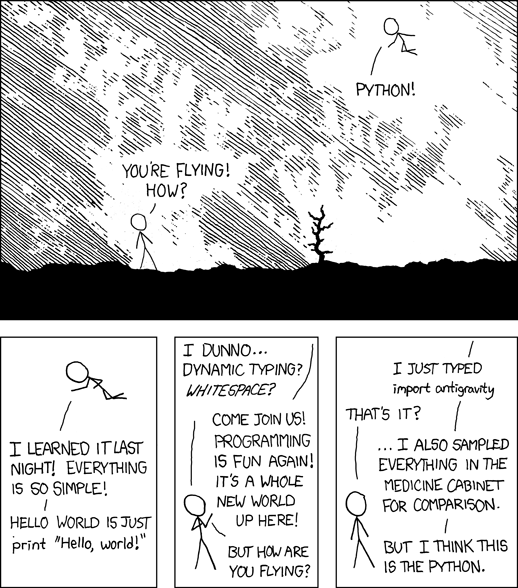
\includegraphics[width=0.5\textwidth]{pictures/xkcd_python.png}
  \caption{\label{figure:xkcd_python}``Python'' by Randall Munroe \cite{Munroe_python}}
\end{figure}

Ein Modul bindet man mit \lpy{import modulname} in sein Programm ein.
Alle Objekttypen (Klassen, Funktionen und andere Objekte) die \lpy{modulname} bereitstellt, können durch \lpy{modulname.oname} erreicht werden.
\begin{lstlisting}
import math
print( math.sin(math.pi/3.0) )
\end{lstlisting}
Wenn man aus \lpy{modulname} bestimmte Objekte einbinden möchte, nutzt man folgende Codezeile.
\begin{lstlisting}
from modulname import oname1, oname2, ...
\end{lstlisting}
Jetzt kann man auf die Objekte direkt (also ohne das Präfix \lpy{modulname.}) zugreifen.
Wir hatten bereits gesehen, wie man die \PythonDrei Printfunktion in \PythonZwei einbinden kann.
\begin{lstlisting}
from __future__ import print_function
\end{lstlisting}
Hier noch ein Beispiel.
\begin{lstlisting}
from math import sin, cos, pi
print( sin(pi/3.0), cos(pi/3.0) )
\end{lstlisting}

An dieser Stelle machen wir noch auf Abschnitt \ref{section:module:empfohlene_module} indem wir eine Hand voll \Python-Pakete erwähnen, die wir oft benutzen.


\subsection{Workflow}
\label{section:crashkurs:workflow}
Wir arbeiten recht erfolgreich mit folgendem Workflow.

Beginne ein Projekt in \Python.
Solange du noch nicht fertig bist:
Wenn eine Funktion zu aufwendig zu implementieren ist, suche nach einer bereits vorhandene \Python Bibliothek (es gibt bestimmt eine).
Wenn eine Funktion für dein Projekt zu langsam ist, schreibe sie in \CC und binde sie als Modul ein.
Wie genau letzteres geht, lernen wir noch.
